\documentclass[11pt,compress,t,notes=noshow, xcolor=table]{beamer}
\usepackage[]{graphicx}\usepackage[]{color}
% maxwidth is the original width if it is less than linewidth
% otherwise use linewidth (to make sure the graphics do not exceed the margin)
\makeatletter
\def\maxwidth{ %
  \ifdim\Gin@nat@width>\linewidth
    \linewidth
  \else
    \Gin@nat@width
  \fi
}
\makeatother

\definecolor{fgcolor}{rgb}{0.345, 0.345, 0.345}
\newcommand{\hlnum}[1]{\textcolor[rgb]{0.686,0.059,0.569}{#1}}%
\newcommand{\hlstr}[1]{\textcolor[rgb]{0.192,0.494,0.8}{#1}}%
\newcommand{\hlcom}[1]{\textcolor[rgb]{0.678,0.584,0.686}{\textit{#1}}}%
\newcommand{\hlopt}[1]{\textcolor[rgb]{0,0,0}{#1}}%
\newcommand{\hlstd}[1]{\textcolor[rgb]{0.345,0.345,0.345}{#1}}%
\newcommand{\hlkwa}[1]{\textcolor[rgb]{0.161,0.373,0.58}{\textbf{#1}}}%
\newcommand{\hlkwb}[1]{\textcolor[rgb]{0.69,0.353,0.396}{#1}}%
\newcommand{\hlkwc}[1]{\textcolor[rgb]{0.333,0.667,0.333}{#1}}%
\newcommand{\hlkwd}[1]{\textcolor[rgb]{0.737,0.353,0.396}{\textbf{#1}}}%
\let\hlipl\hlkwb

\usepackage{framed}
\makeatletter
\newenvironment{kframe}{%
 \def\at@end@of@kframe{}%
 \ifinner\ifhmode%
  \def\at@end@of@kframe{\end{minipage}}%
  \begin{minipage}{\columnwidth}%
 \fi\fi%
 \def\FrameCommand##1{\hskip\@totalleftmargin \hskip-\fboxsep
 \colorbox{shadecolor}{##1}\hskip-\fboxsep
     % There is no \\@totalrightmargin, so:
     \hskip-\linewidth \hskip-\@totalleftmargin \hskip\columnwidth}%
 \MakeFramed {\advance\hsize-\width
   \@totalleftmargin\z@ \linewidth\hsize
   \@setminipage}}%
 {\par\unskip\endMakeFramed%
 \at@end@of@kframe}
\makeatother

\definecolor{shadecolor}{rgb}{.97, .97, .97}
\definecolor{messagecolor}{rgb}{0, 0, 0}
\definecolor{warningcolor}{rgb}{1, 0, 1}
\definecolor{errorcolor}{rgb}{1, 0, 0}
\newenvironment{knitrout}{}{} % an empty environment to be redefined in TeX

\usepackage{alltt}
\newcommand{\SweaveOpts}[1]{}  % do not interfere with LaTeX
\newcommand{\SweaveInput}[1]{} % because they are not real TeX commands
\newcommand{\Sexpr}[1]{}       % will only be parsed by R



\usepackage[english]{babel}
\usepackage[utf8]{inputenc}

\usepackage{dsfont}
\usepackage{verbatim}
\usepackage{amsmath}
\usepackage{amsfonts}
\usepackage{bm}
\usepackage{csquotes}
\usepackage{multirow}
\usepackage{longtable}
\usepackage{booktabs}
\usepackage{enumerate}
\usepackage[absolute,overlay]{textpos}
\usepackage{psfrag}
\usepackage{algorithm}
\usepackage{algpseudocode}
\usepackage{eqnarray}
\usepackage{arydshln}
\usepackage{tabularx}
\usepackage{placeins}
\usepackage{tikz}
\usepackage{setspace}
\usepackage{colortbl}
\usepackage{mathtools}
\usepackage{wrapfig}
\usepackage{bm}
\usetikzlibrary{shapes,arrows,automata,positioning,calc,chains,trees, shadows}
\tikzset{
  %Define standard arrow tip
  >=stealth',
  %Define style for boxes
  punkt/.style={
    rectangle,
    rounded corners,
    draw=black, very thick,
    text width=6.5em,
    minimum height=2em,
    text centered},
  % Define arrow style
  pil/.style={
    ->,
    thick,
    shorten <=2pt,
    shorten >=2pt,}
}
\usepackage{subfig}


% Defines macros and environments
\input{../../style/common.tex}
% \input{common.tex}

%\usetheme{lmu-lecture}
\newcommand{\titlefigure}{figure/eval_test_3}
\newcommand{\learninggoals}{
\item Understand the definition of test error
\item Understand how overfitting can be seen in the test error}
\usepackage{../../style/lmu-lecture}

\let\code=\texttt
\let\proglang=\textsf

\setkeys{Gin}{width=0.9\textwidth}

\title{Introduction to Machine Learning}
% \author{Bernd Bischl, Christoph Molnar, Daniel Schalk, Fabian Scheipl}
\institute{\href{https://compstat-lmu.github.io/lecture_i2ml/}{compstat-lmu.github.io/lecture\_i2ml}}
\date{}

\setbeamertemplate{frametitle}{\expandafter\uppercase\expandafter\insertframetitle}

\begin{document}

% This file loads R packages, configures knitr options and sets preamble.Rnw as parent file
% IF YOU MODIFY THIS, PLZ ALSO MODIFY setup.Rmd ACCORDINGLY...

% Defines macros and environments
\input{../../latex-math/basic-math.tex}
\input{../../latex-math/basic-ml.tex}
%! includes: evaluation-train

\lecturechapter{Evaluation: Test Error}
\lecture{Introduction to Machine Learning}

% \begin{vbframe}{Test Error and Hold-Out Splitting}
% To measure performance, let’s simulate how our model will be applied on new, unseen data.\\
% \lz
% $\rightarrow$ Predict only on data not used during training and measure performance there.\\[.5em]
% $\rightarrow$ For a given set $D$, we have to preserve some data for testing that we cannot use for training.
% \end{vbframe}

% ------------------------------------------------------------------------------

% \begin{vbframe}{Test Error}
% 
% % FIGURE SOURCE: https://docs.google.com/drawings/d/1q7WN1_YKHedIPNySiZBEraLtTkHRX12Ej6M6ISbfMD0/edit?usp=sharing
% 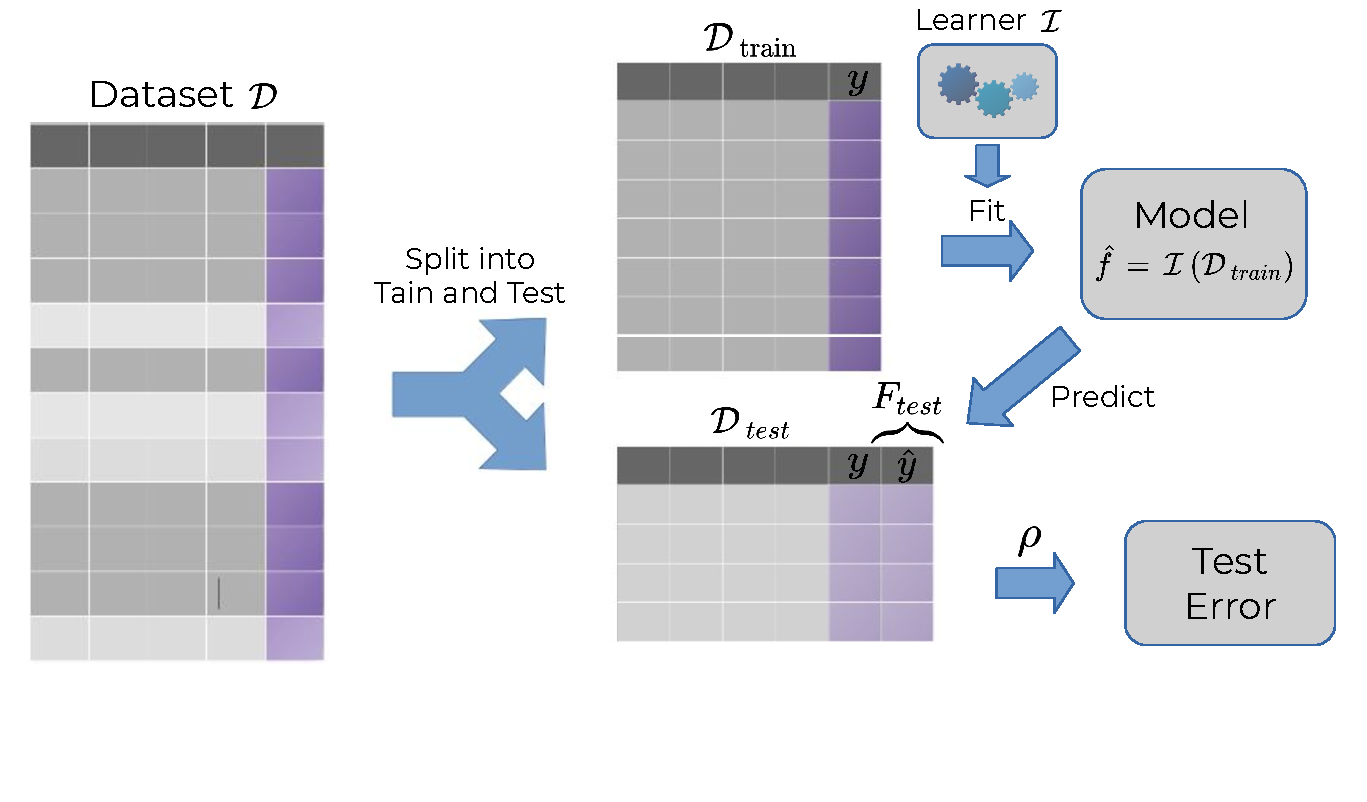
\includegraphics[width=0.8\textwidth, trim=270 0 0 0, clip]{figure_man/test_error.pdf}
% 
% \end{vbframe}

% ------------------------------------------------------------------------------

\begin{vbframe}{Test Error and Hold-Out Splitting}

% \begin{itemize}
% \item The fundamental idea behind test error estimation (and everything that will follow) is quite simple
% \item To measure performance, let’s simulate how our model will be applied on new, unseen data
% \item So, to evaluate a given model do exactly that, predict only on data not used during training and measure performance there
% \item That implies that for a given set D , we have to preserve some data for testing that we cannot use for training
% \end{itemize}

\begin{itemize}
  \item In order to avoid optimistic bias we will use the 
  \textbf{test error} to simulate how our model performs on new, unseen data.
  \item Evaluating a given model therefore means predicting only on the
  test data and measuring the resulting performance.
  \item This implies splitting the data into disjoint sets (e.g., 2/3 for 
  training and 1/3 for testing).
\end{itemize}

\begin{center}
  % FIGURE SOURCE: https://docs.google.com/drawings/d/1q7WN1_YKHedIPNySiZBEraLtTkHRX12Ej6M6ISbfMD0/edit?usp=sharing
  %resampling brackets are cut out
  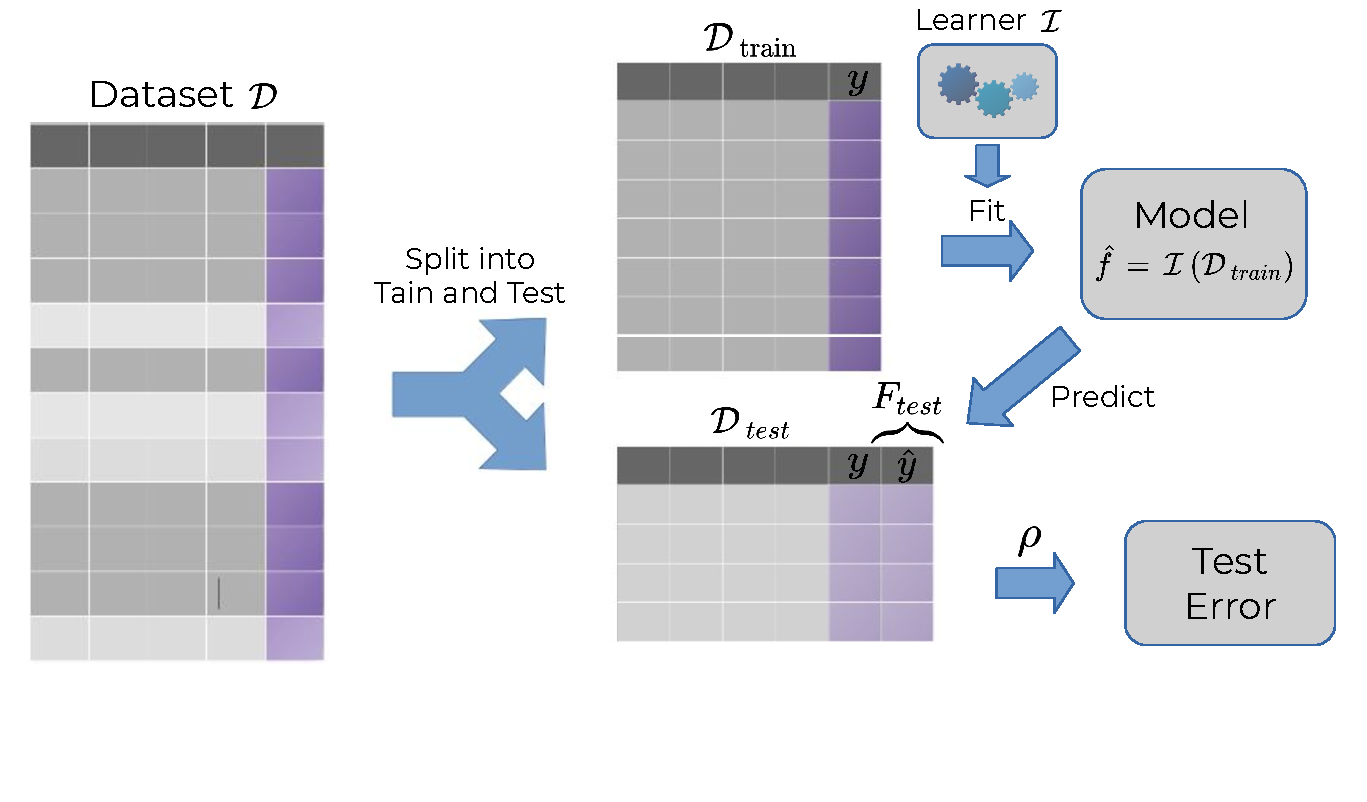
\includegraphics[width=0.8\textwidth]{figure_man/test_error.pdf}
\end{center}

\end{vbframe}

% ------------------------------------------------------------------------------

% \begin{vbframe}{Test Error and Hold-Out Splitting}
% \begin{itemize}
%   \item Split data into 2 parts, e.g., 2/3 for training, 1/3 for testing
%   \item Evaluate on data not used for model building
% \end{itemize}
% 
% % FIGURE SOURCE: https://docs.google.com/drawings/d/1q7WN1_YKHedIPNySiZBEraLtTkHRX12Ej6M6ISbfMD0/edit?usp=sharing
% 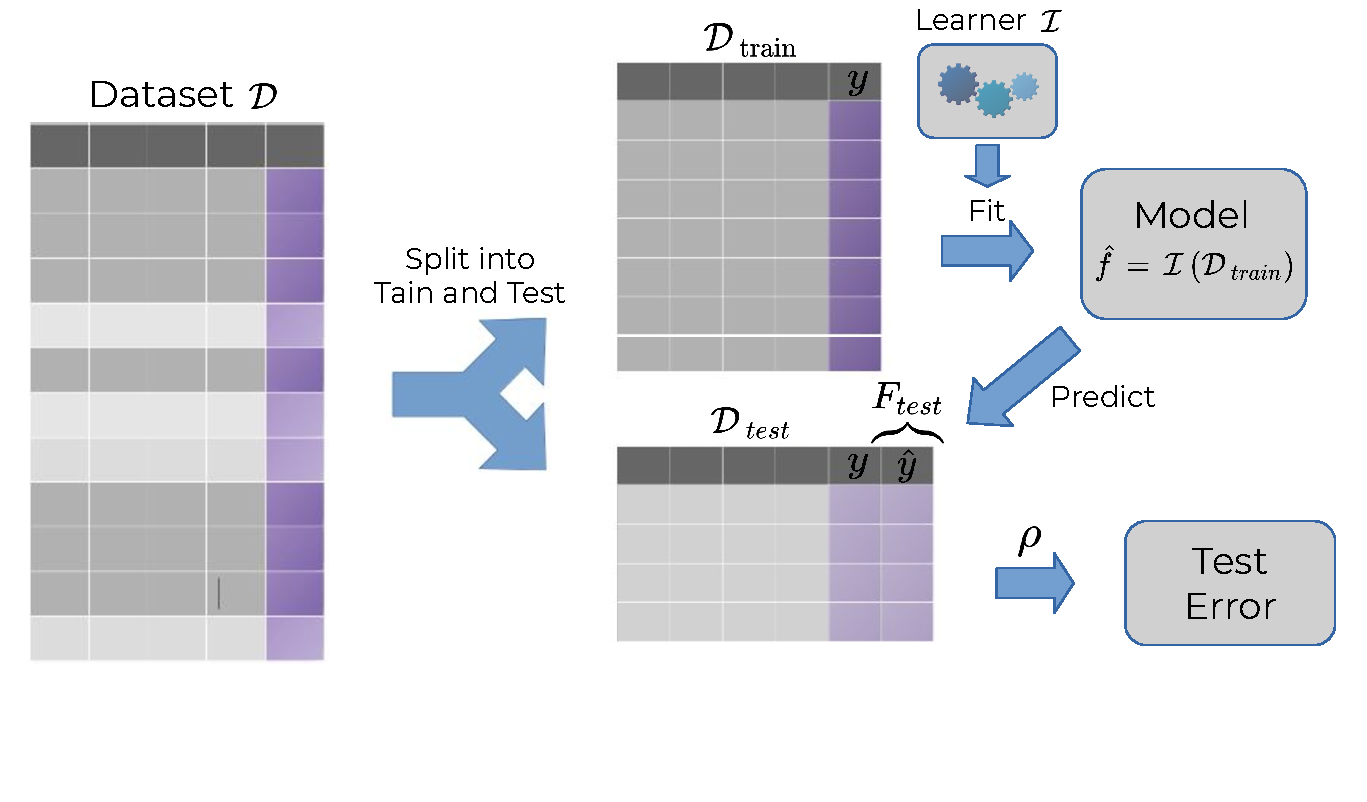
\includegraphics[width=\textwidth]{figure_man/test_error.pdf}
% 
% \end{vbframe}

% ------------------------------------------------------------------------------

\begin{vbframe}{Example: Polynomial Regression}

Consider the previous example with the sinusoidal function
$0.5 + 0.4 \cdot \sin (2 \pi x) + \epsilon$:

\vfill

\begin{center}
  \includegraphics[width=0.85\textwidth]{figure/eval_train_1}
\end{center}

Again, we approximate the data with a $d^{th}$-degree polynomial:
\[ \fxt = \theta_0 + \theta_1 \xv + \cdots + \theta_d \xv^d = \sum_{j = 0}^{d}
\theta_j \xv^j\text. \]

\framebreak

\includegraphics[width=0.8\textwidth]{figure/eval_test_2} 

\begin{itemize}
  \footnotesize
  \item $d = 1$: MSE = 0.038: clearly underfitting
  \item $d = 3$: MSE = 0.002: pretty OK
  \item $d = 9$: MSE = \textcolor{blue}{0.046}: clearly overfitting
\end{itemize}

\vfill

While the training error monotonically decreases for rising $d$, 
the test error reflects the fact that higher-degree polynomials overfit 
the data.

\end{vbframe}

% ------------------------------------------------------------------------------

% \begin{vbframe}{Test Error}
% 
% Let's consider the following example:\\
% Sample data from sinusoidal function
% $0.5 + 0.4 \cdot \sin (2 \pi x) + \epsilon$\\
% \lz
% \begin{knitrout}\scriptsize
% \definecolor{shadecolor}{rgb}{0.969, 0.969, 0.969}\color{fgcolor}
% 
% {\centering \includegraphics[width=0.8\textwidth]{figure/eval_test_1} 
% 
% }
% 
% 
% 
% \end{knitrout}
% Try to approximate with a $d^{th}$-degree polynomial:
% \[ \fxt = \theta_0 + \theta_1 x + \cdots + \theta_d x^d = \sum_{j = 0}^{d} \theta_j x^j\text{.} \]
% \end{vbframe}
% 
% % ------------------------------------------------------------------------------

% \begin{vbframe}{Test Error}
% \begin{knitrout}\scriptsize
% \definecolor{shadecolor}{rgb}{0.969, 0.969, 0.969}\color{fgcolor}
% 
% {\centering \includegraphics[width=0.95\textwidth]{figure/eval_test_2}
% 
% }
% 
% 
% 
% \end{knitrout}
% 
% \begin{itemize}
% \item d=1: MSE = 0.038: Clear underfitting
% \item d=3: MSE = 0.002: Pretty OK
% \item d=9: MSE = 0.046: Clear overfitting
% \end{itemize}
% 
% \end{vbframe}

% ------------------------------------------------------------------------------

\begin{vbframe}{Test Error}

Plot evaluation measure for all polynomial degrees:

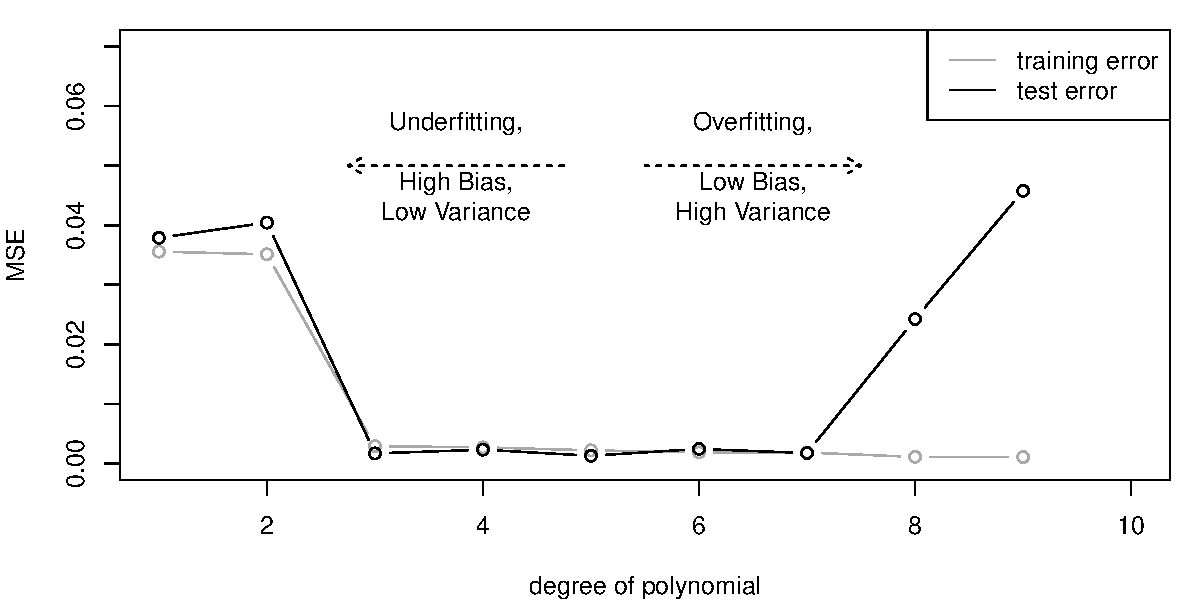
\includegraphics[width=0.9\textwidth]{figure/eval_test_3} 

Increasing model complexity tends to cause

\begin{itemize}
  \item a decrease in training error, and\\
  \item a U-shape in test error\\ 
  (first underfit, then overfit, sweet-spot in the middle).
  \end{itemize}
  
\end{vbframe}

% ------------------------------------------------------------------------------

\begin{vbframe}{Training vs. test error}
\begin{small}
\begin{itemize}
\item We take the Boston Housing data set where the value of houses in the area around Boston is predicted based on $13$ features describing the region (e.g., crime rate, name of the town, etc. ).
\item We fit a polynomial regression model on it $$ \yv_{medv} = \beta_0 + \sum_{j=0}^d \sumin \beta_{i}^j \xv_i= \beta_0 + \sum_{j=0}^d \sumin \beta_{1} \xv_{1} + \beta_{1}\xv_{1}^2+ ... + \beta_{1}\xv_{1}^d +  ... + \beta_{n} \xv_{n}^d$$
with $n$ features and $d$ degrees polynomials.
\item We observe the train and test error, if we change the size of training set, the size of the test set and the model complexity (incresing the possible degrees of the polynomials). 
\end{itemize}

\vfill

\textbf{The training error...}

\begin{itemize}
  \item is a biased estimator as performance is measured on the same data the 
  model was trained on.
\end{itemize}

\framebreak

\textbf{The training error...}
\begin{itemize}
  \item decreases with smaller training set size as it becomes easier for the 
  model to learn all observed patterns perfectly.
\end{itemize}
\end{small}
\begin{center}
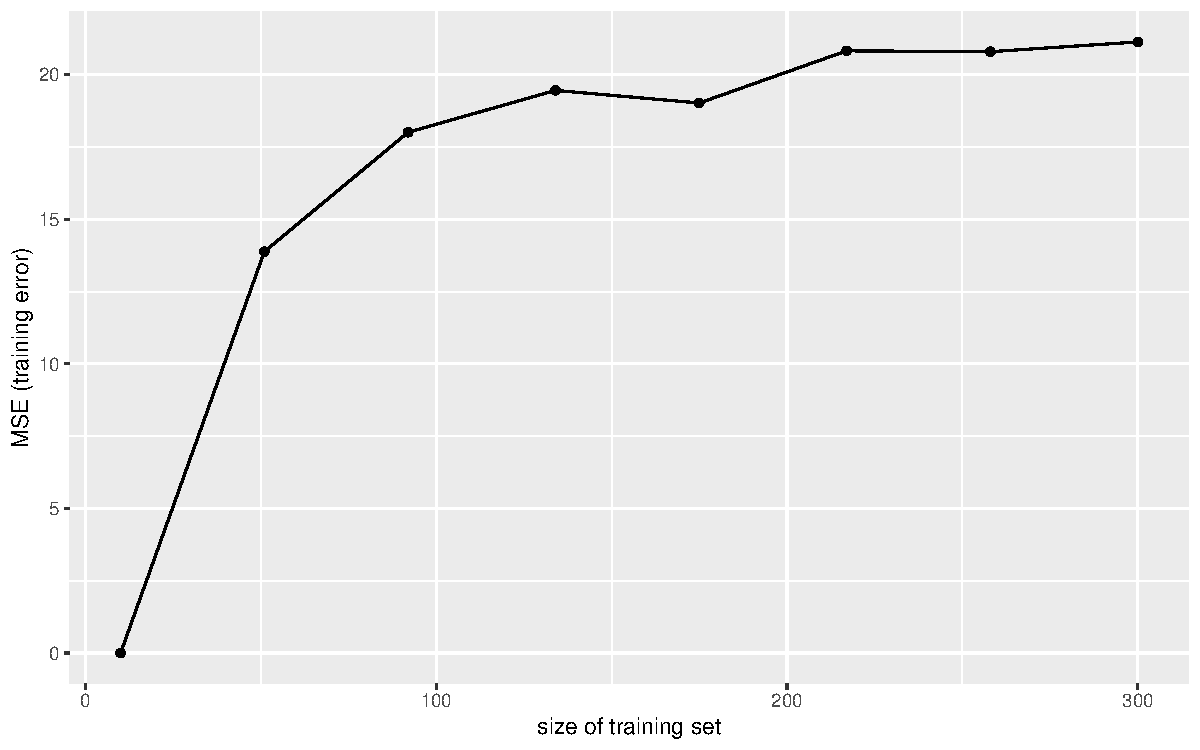
\includegraphics[width=0.7\textwidth]{figure/fig-train-vs-test-error-1}
\end{center}

\framebreak

\textbf{The training error...}
\begin{itemize}  
  \item decreases with increasing model complexity as the model gets better at
  learning more complex structures (here: more degrees in polynomial regression).
\end{itemize}

\begin{center}
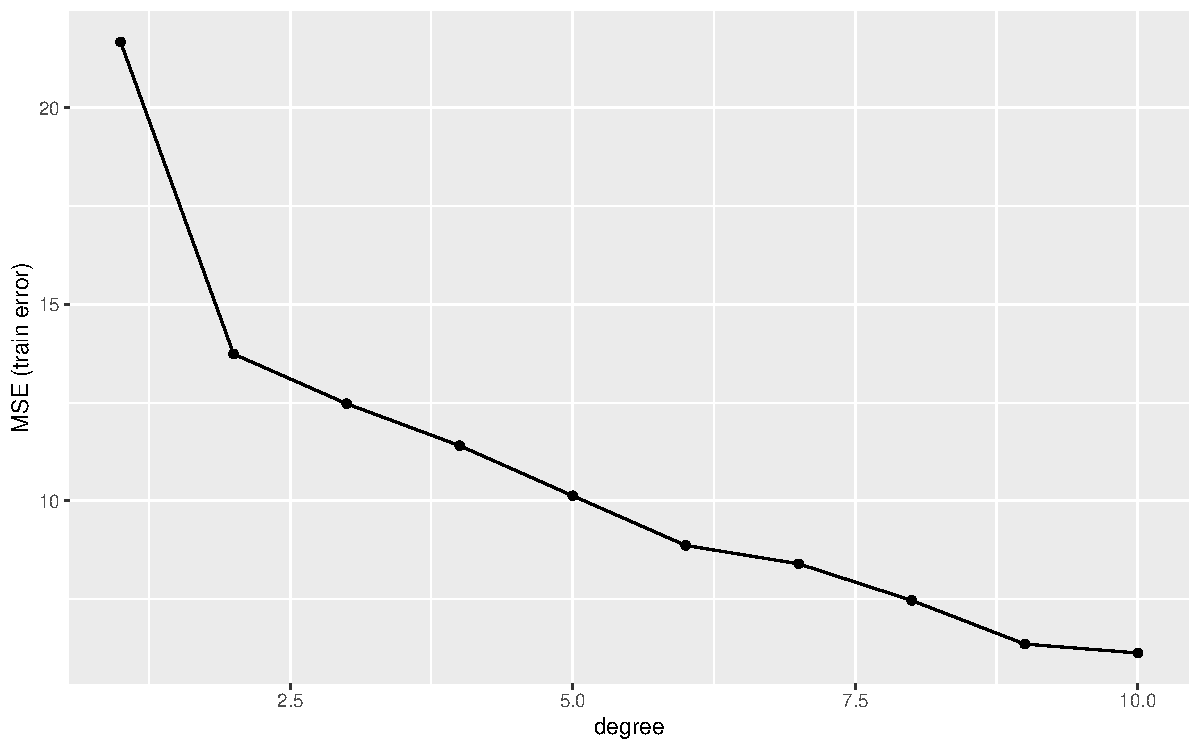
\includegraphics[width=0.7\textwidth]{figure/fig-train-vs-test-error-4}
\end{center}

\framebreak

\textbf{The test error...}

\begin{itemize}
  \item will typically decrease with larger training set size as the model 
  generalizes better with more data to learn on.
  
\end{itemize}
\begin{center}
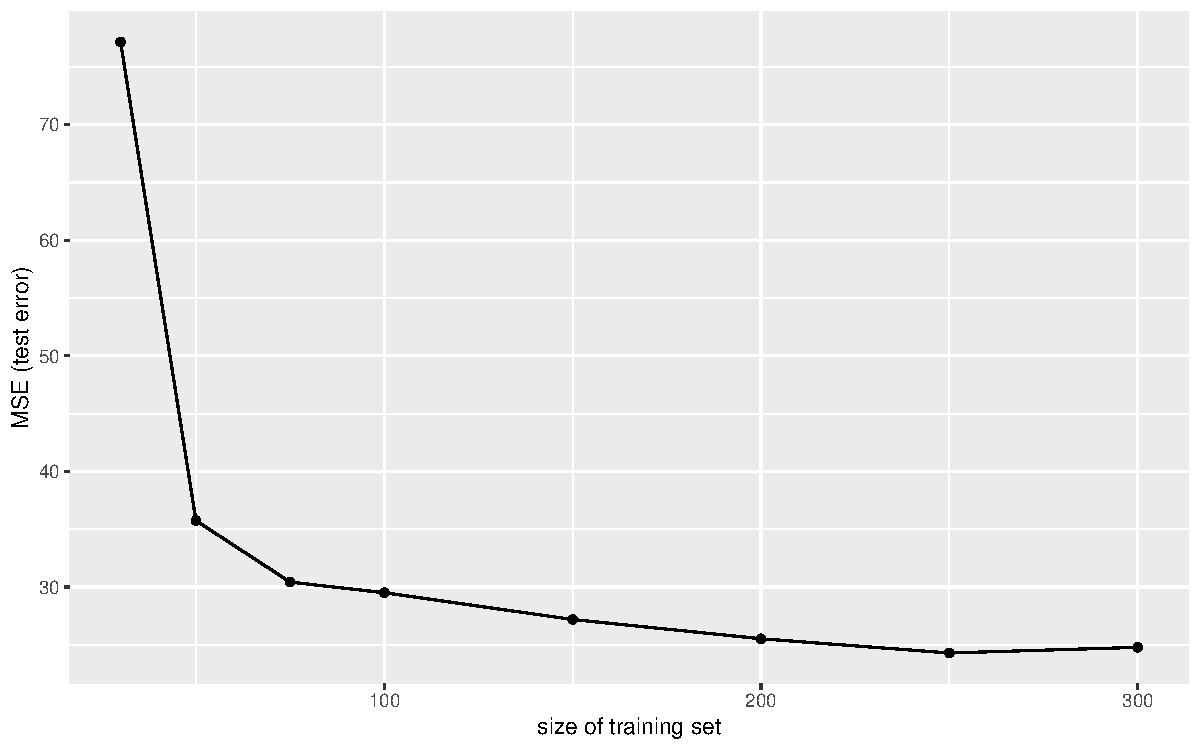
\includegraphics[width=0.8\textwidth]{figure/fig-train-vs-test-error-2}
\end{center} 

\framebreak
\textbf{The test error...}

\begin{itemize}  
  
  \item will have higher variance with smaller test set size.

\end{itemize}
\begin{center}
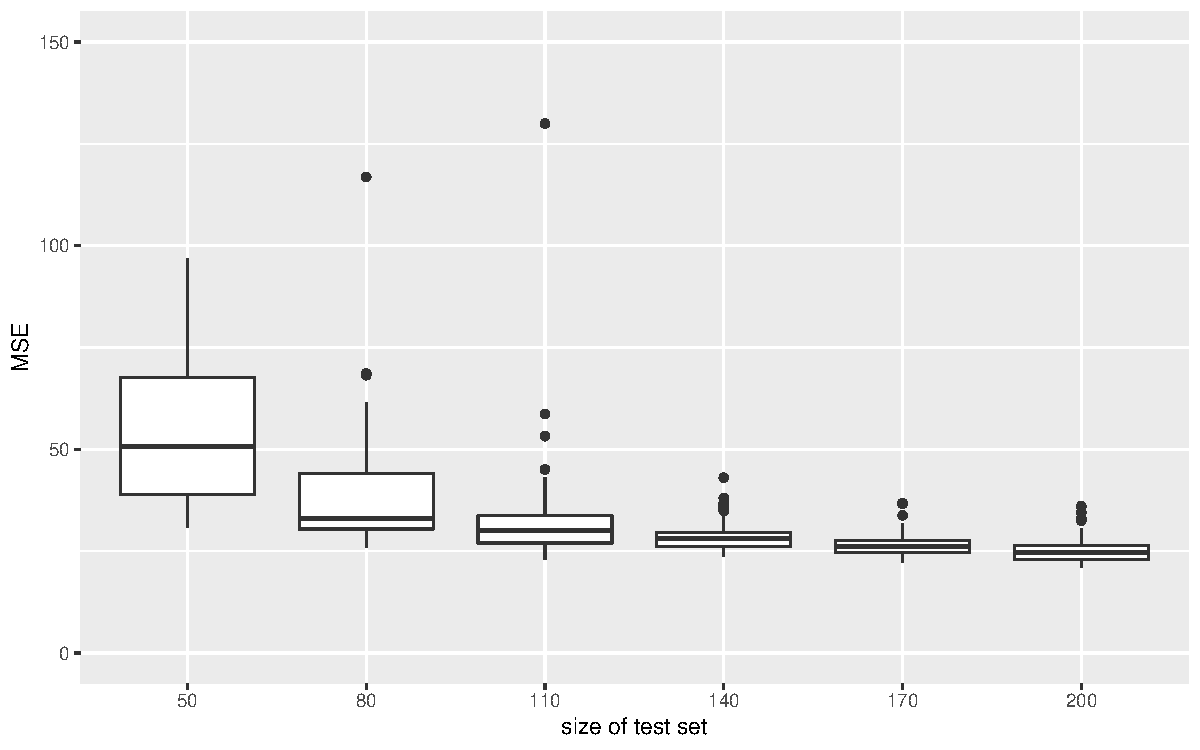
\includegraphics[width=0.8\textwidth]{figure/fig-train-vs-test-error-3}
\end{center}  

\framebreak
\textbf{The test error...}

\begin{itemize}    
  
  \item will have higher variance with increasing model complexity (here: more degrees in polynomial regression).
\end{itemize}

\begin{center}
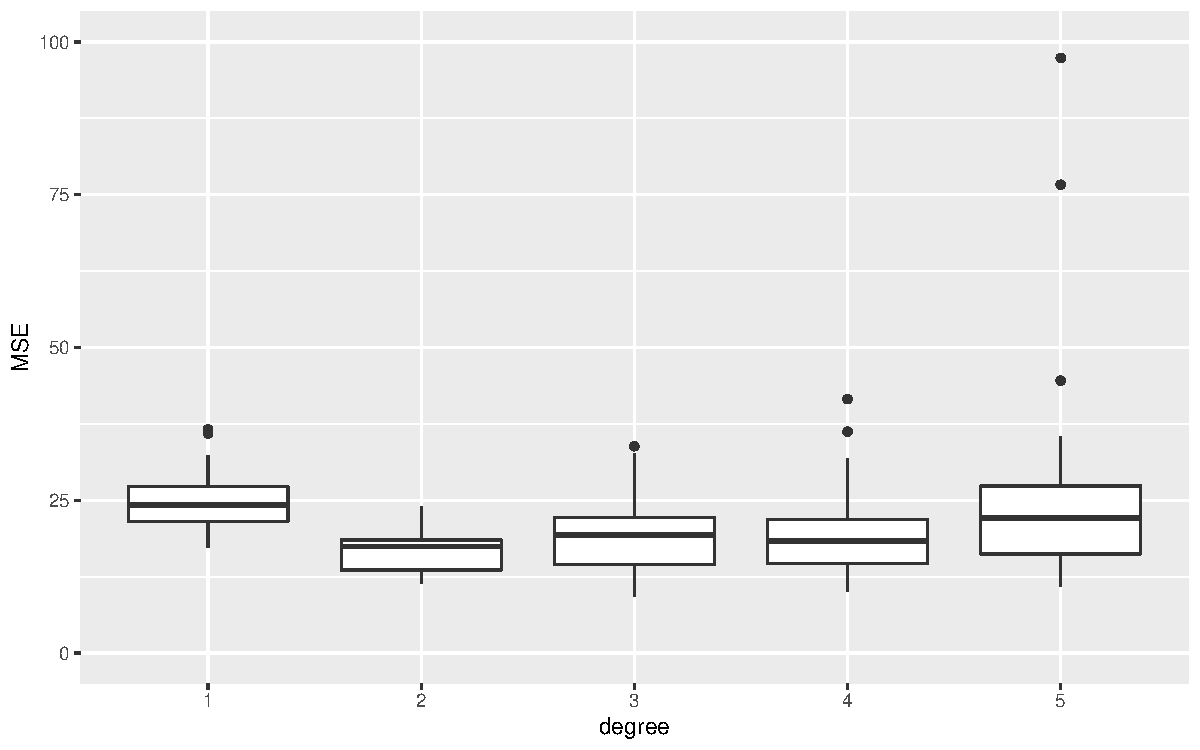
\includegraphics[width=0.8\textwidth]{figure/fig-train-vs-test-error-5}
\end{center} 

\end{vbframe}


% ------------------------------------------------------------------------------

\begin{vbframe}{Test error Problems}

\begin{itemize}
  \item In general, the test error is a good estimator of future performance,
  \textbf{given} the test data and data we might see in future applications are 
  indeed \textit{iid} samples from the same underlying distribution.
  \item Hold-out sampling produces a trade-off between \textbf{bias} and
  \textbf{variance} that is balanced by the split ratio.
  % \begin{itemize}
  %   \item Smaller training set $\rightarrow$ poor fit, high bias in error 
  %   estimate.
  %   \item Smaller test set $\rightarrow$ high variance in error estimate.
  % \end{itemize}   
  \item \textbf{Sample size} plays a crucial role in deciding on a split 
  strategy:
  \begin{itemize}
    \item If the size of our initial, complete data set $\D$ is limited,
    single train-test splits can be problematic.
    \item Small-sample problems come in different shapes in ML -- 
    maybe overall set size is sufficient but one of the classes is very small.
  \end{itemize}
  \item It is generally advisable to try out different train-test splits and 
  study the resulting error measurement fluctuation.
\end{itemize}

\framebreak

We simulate repeated $\tfrac{2}{3}$ / $\tfrac{1}{3}$ train-test splits on two ML 
tasks:\\ 
\texttt{iris} ($n$ = 150) and \texttt{sonar} ($n$ = 208).\\
So we have about 50 (\texttt{iris}) and 70 (\texttt{sonar}) observations in our 
respective test sets.\\

\vfill

The plots below show the strong variation in test errors (50 
repetitions).

\vfill

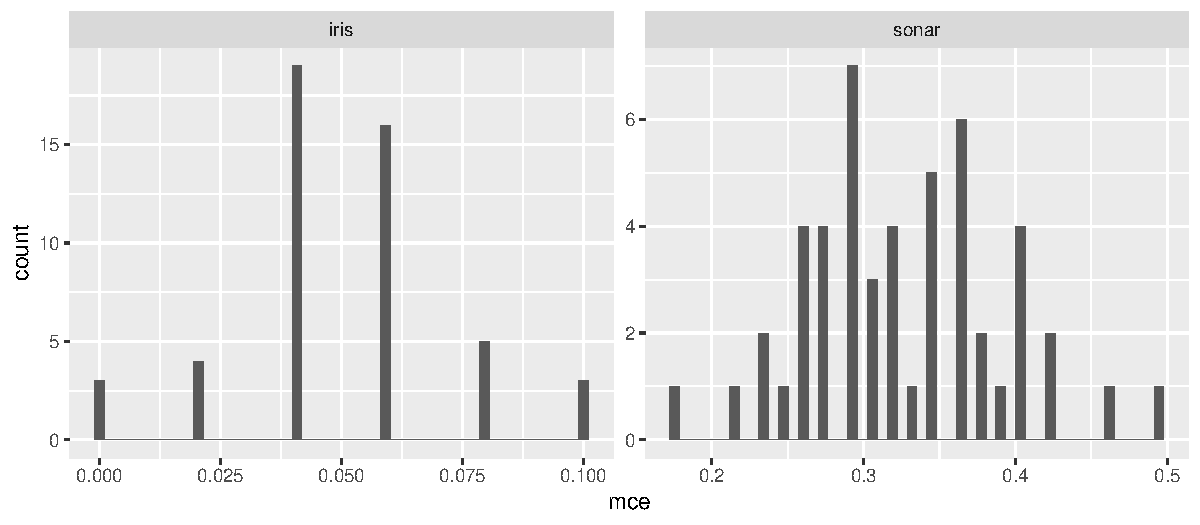
\includegraphics[width=\textwidth]{figure/test-error-flucuation} 

\end{vbframe}

% ------------------------------------------------------------------------------

% \begin{vbframe}{Training vs. test error}
%   \vspace{-0.25cm}
%   \begin{blocki}{The training error}
%   \vspace{-0.25cm}
%     \item is an over-optimistic (biased) estimator as the performance is measured on the same data the learned model was trained for
%     \item decreases with smaller training set size as it is easier for the model to learn the underlying structure in the training set perfectly
%     \item decreases with increasing model complexity as the model is able to learn more complex structures
%   \end{blocki}
%   \vspace{-0.25cm}
%   \begin{blocki}{The test error}
%   \vspace{-0.25cm}
%   \item will typically decrease when the training set increases as the model generalizes better with more data (more data to learn)
%   \item will have higher variance with decreasing test set size
%   \item will have higher variance with increasing model complexity
%   \end{blocki}
% \end{vbframe}

% ------------------------------------------------------------------------------

% Visualize the perfomance estimator - and the MSE of the estimator - in relation to the true error rate.

% \begin{vbframe}{Bias-Variance of Hold-Out}
% \begin{itemize}
% \item If the size of our initial, complete data set $\D$ is limited,
%   single train-test splits can be problematic.
% \item The smaller our single test set is, the higher the variance
%   of our estimated performance error (e.g., if we test on one observation, in the extreme case).
%   But note that by just making the test set smaller, we do not introduce any bias,
%   as we simply average losses on i.i.d. observations from $\Pxy$.
% \item The smaller our training set becomes, the more pessimistic bias we introduce into the model.
%   Note that if $|D| = n$, our aim is to estimate the performance of a model fitted
%   on $n$ observations (as this is what we will do in the end). If we fit on less data during
%   evaluation, our model will learn less, and perform worse. Very small training sets will also
%   increase variance a bit.
% \end{itemize}
% \end{vbframe}

% ------------------------------------------------------------------------------

\begin{vbframe}{Bias-Variance of Hold-Out -- Experiment}

\begin{itemize}
  \item Data: simulate \texttt{spirals} data ($sd = 0.1$) from \texttt{mlbench}.
  \item Learner: CART (\texttt{classif.rpart} from \texttt{mlr3}).
  \item Goal: estimate real performance of a model with $|\Dtrain| = 500$.
  \begin{itemize}
    \item Get the "true" estimator by repeatedly sampling 500 observations from 
    the simulator, fit the learner, then evaluate on $10^5$ observations -- 
    obviously not feasible in practice.
    \item Analyze different split rates $s \in \{0.05, 0.10, ..., 0.95\}$ 
    with $|\Dtrain| = s \cdot 500$.
    \item Estimate performance on $\Dtest$ with $|\Dtest| = (1 - s) \cdot 500$.
    \item Repeat the experiment 50 times for each split rate.
  \end{itemize}
\end{itemize}

\framebreak

%test-holdout-example

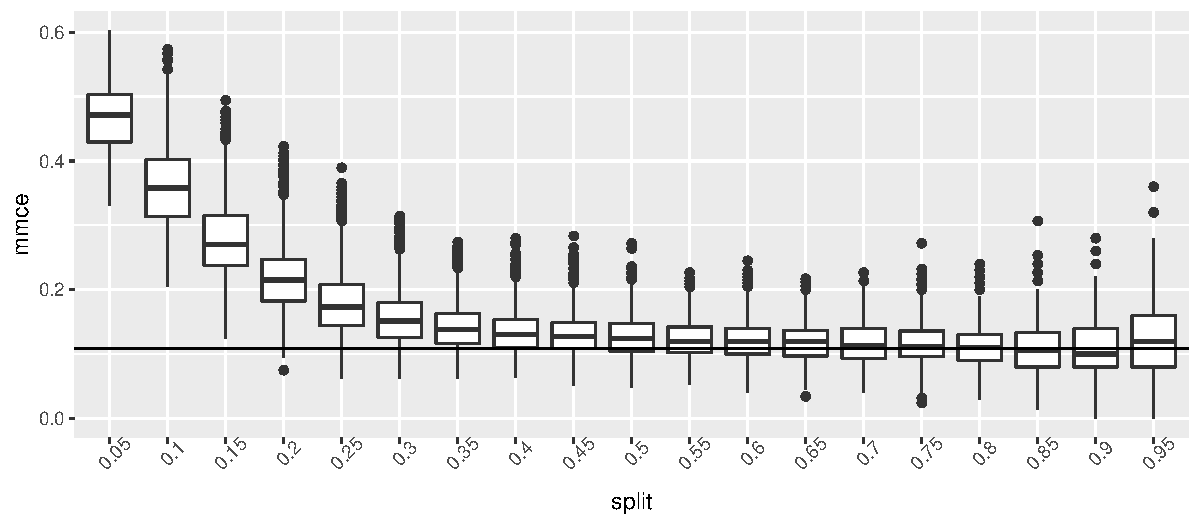
\includegraphics[width=\textwidth]{figure/test-holdout-example} 

\lz

\begin{itemize}
  \item We clearly see the pessimistic bias for small training sets -- we cannot 
  learn much from substantially fewer than 500 observations. 
  \item At the same time, we observe an increase in variance when test sets 
  become smaller.
\end{itemize}

\framebreak

\begin{itemize}
  \item We now plot the MSE between true performance (horizontal line in 
  previous plot) and hold-out values in each boxplot.
  \item The split rate with the lowest MSE value produces the best estimator, 
  which is pretty close to a training set ratio of 2/3.
  \item NB: this is a single experiment and not a scientific study, but this 
  rule-of-thumb has also been validated in larger studies.
\end{itemize}

% test-holdout-example
\begin{center}
  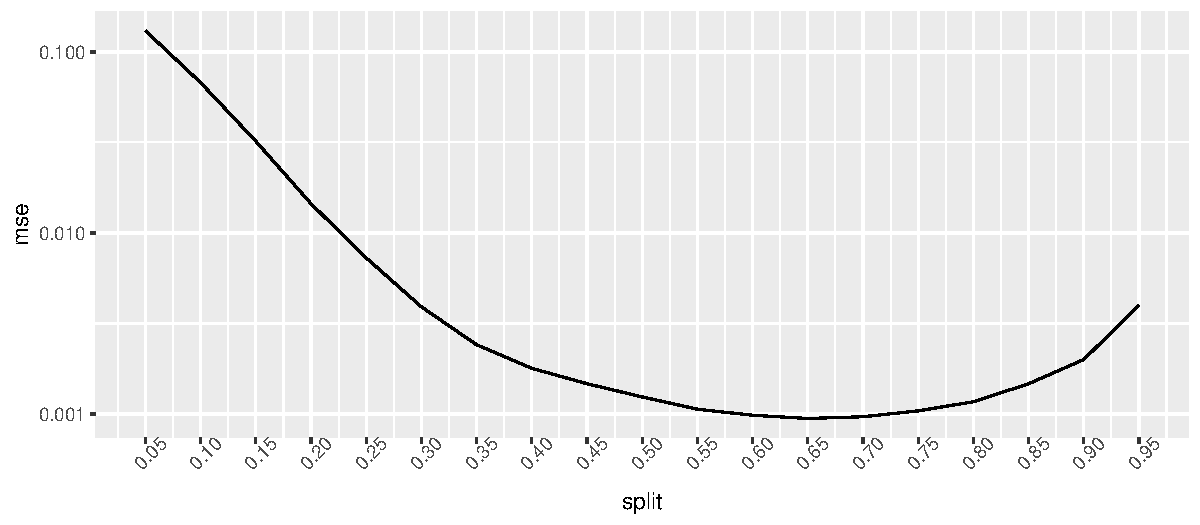
\includegraphics[width=0.9\textwidth]{figure/test-holdout-example-2} 
\end{center}

\end{vbframe}

% ------------------------------------------------------------------------------

\begin{vbframe}{Test error}

To clear up a major point of confusion:
\medskip

\begin{itemize}
  \item In ML we frequently face a weird situation.
  \item We are usually given a single data set, and at the end of our model 
  selection and evaluation process, we will likely fit one model on exactly that 
  complete data set. 
  \item As training error evaluation does not work, we have no other option but 
  to evaluate exactly that model.
  \item Hold-out splitting (and \textbf{resampling}) are tools to estimate 
  future performance in a valid manner. 
  \item All of the models produced during that phase of evaluation are only
  intermediate results.
\end{itemize}

\end{vbframe}

% ------------------------------------------------------------------------------

\endlecture
\end{document}
